\documentclass{./../../Latex/handout}
\begin{document}
\thispagestyle{plain}
\myheader{Linear Regression Model: Functional Forms}

Consider the fitted line from a linear model:
 $$ \hat{Y} = \hat{\beta}_0 + \hat{\beta}_1 X $$
 
To determine how $\hat{Y}$ changes due to a one-unit change in $X$, we can differentiate the above equation with respect to $X$:
  $$ \frac{d\hat{Y}}{d X} =  \hat{\beta}_1 $$

Here, $d X$ denotes a small change in $X$.

So $\hat{\beta}_1$ represents the change in $\hat{Y}$ due to a one-unit change in $X$. To see this note that we can rewrite the above expression as:
 $$d\hat{Y}=  \hat{\beta}_1 \cdot dX$$
Therefore, if $dX=1$, then $d\hat{Y}= \hat{\beta}_1$. \\

\fbox{\begin{minipage}{\textwidth}
Quick Reminder: Rules of Differentiation\footnote{If you need a refresher, refer to the handout on reviewing calculus. } 
\begin{itemize}
\item $y=a$, $ \dfrac{dy}{dx}=0$
\item $y=ax$, $\dfrac{dy}{dx}=a$
\item $y=ax^b$, $\dfrac{dy}{dx}=abx^{b-1}$
\item $y=log(x)$, $\dfrac{dy}{dx}=\dfrac{1}{x}$
\item $z=f(y), y=g(x)$,  $\dfrac{d z}{d x}=\dfrac{d z}{d y} \cdot \dfrac{d y}{d x}$
\end{itemize}
\end{minipage}} 

%%%%%%%%%%%%%%%%%%%%%%%%% Quadratic Functional Form
\section{Quadratic Functional Form}
 
There are cases where a linear line may not be the optimal way to represent data, particularly when the effect of $X$ on $Y$ is not constant and varies with $X$. We saw this was the case when fitting wages as a function of age in class, as wage growth may be higher for workers in their 20s and 30s than for those in their 40s and 50s. To address this, we can fit a curve, such as a quadratic function.  OLS now minimizes the sum of squared residuals between the data and the quadratic function. (Note that the model still has to be linear in parameters, after all, it is the \textit{linear} regression model.)

 To fit a quadratic model, we can estimate the following equation: 
 $$ \hat{Y} =  \hat{\beta}_0 + \hat{\beta_1} X + \hat{\beta}_2 X^2  $$

To determine how $\hat{Y}$ changes due to a one-unit change in $X$ in this model, we can differentiate the equation as before:
  $$ \frac{d\hat{Y}}{d X} =  \hat{\beta}_1 + 2 \hat{\beta}_2 X $$
This indicates that the change in $\hat{Y}$ with respect to $X$ now changes with $X$ due to the quadratic term. In other words, the slope of the curve, as represented by the derivative, changes with $X$. \\
 
\textit{Example: Effect of Age on Wages} \\~\\
Here is the equation of the curve fitted from a regression analysis of wages on age using the ACS 2019 data.
$$ \hat{wages} = -52207 + 4775.64 \cdot age -49.5 \cdot age^2   $$

The corresponding plot for the fitted curve is presented in Figure 1. The plot indicates that the model predicts a positive relationship between wages and age; however, this effect becomes weaker for older individuals.

\begin{figure*}[t]\caption{Fitted Relationship between Wages and Age}
\centering
	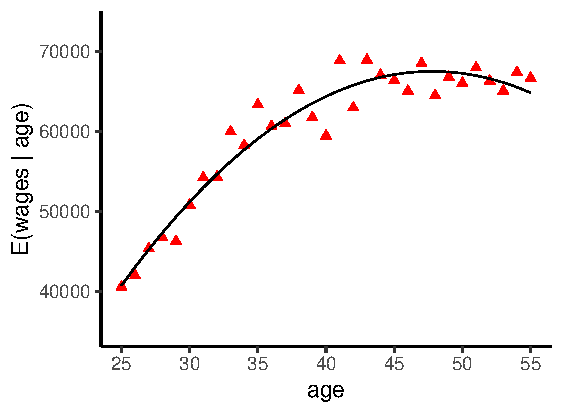
\includegraphics{./../../output/scatter_age_wage_qfit.pdf}	
\end{figure*}

Note that the intercept term is negative, but it is not meaningful since there are no individuals in the sample with an age of 0. 

The change in wages associated with a one-unit change in age is given by: $$ \frac{d \ \hat{wages}}{d \ age} = 4775.64 - 2 \times 49.5 age$$ 

Therefore, the effect of age on wages changes with age itself; specifically in this case, it decreases with age due to the negative coefficient on the quadratic term.

For example, going from 30 to 31 years of age would result in a change in wages of $4775.64 - 2 \times 49.5 \cdot 30 = \$1,805.64$. However, at the age of 40, the change would be only $\$815.64$, and at 50, the change would be $-\$174.36$.

%%%%%%%%%%%%%%%%%%%%%%%%%%%%% Log Functional Forms
 \section{Log Functional Forms}
 
 Logarithmic transformations of variables are often used in statistical analysis, not only to handle outliers and skewed distributions but also because the interpretation of the coefficients changes. When a variable is transformed into log terms, its coefficients can be interpreted as percentage changes, which is useful in economic applications. This is because the derivative of the natural logarithmic function is given by:
 
 $$ \frac{d \log(X)}{dX} = \frac{1}{X}$$
 
This means that we can express the change in the log of $X$ as: 
$$ d \log(X) = \frac{dX}{X} $$
Thus, the change in the log of $X$, denoted as $d\log(X)$, is equivalent to the relative change in $X$, given by $dX/X$. In other words, $d\log(X)$ represents the change in $X$, given by $dX$, relative to its initial value $X$.

This means that we can write the percentage change in $X$ as 100 times $d\log(X)$ because:
 $$ 100 \times d\log(X) = \frac{dX}{X}\times 100 = \text{\% change in $X$} $$
 
\underline{Three possible models:}

% Level-Log
1. \textit{Level-Log Model:}
  $$\hat{Y} = \hat{\beta_0} +  \hat{\beta_1} \log(X)$$
  
To interpret the coefficients, we can differentiate $\hat{Y}$ with respect to $X$:
  $$ \frac{d \hat{Y} }{dX} = \hat{\beta_1} \cdot \frac{1}{X} $$
  
The above holds because the derivative of $\log(X)$ with respect to $X$ is $1/X$. If we rearrange the terms by bringing $X$ to the left-hand side, we get:
$$ \frac{d \hat{Y} }{dX/X} = \hat{\beta_1} $$

So $\hat{\beta_1}$ represents the change in $Y$ relative to the relative change in $X$. Dividing both sides by 100, we get:$$ \frac{d \hat{Y} }{100 \cdot dX/X} = \frac{\hat{\beta_1}}{100} $$

Thus, we can interpret $\hat{\beta_1}/100$ as the unit change in $Y$ relative to a 1\% change in $X$.

Alternatively, we can differentiate $\hat{Y} = \hat{\beta_0} + \hat{\beta_1} \log(X)$ by $\log(X)$ directly:\footnote{Essentially, you are just treating $\log(X)$ as another variable, say $Z=\log(X)$. Then the model is: $\hat{Y} = \hat{\beta_0} + \hat{\beta_1} Z$, and $dY/dZ=\hat{\beta_1}$, but since $Z=\log(X)$, $dY/d\log(X)=\hat{\beta_1}$.}
$$ \frac{d \hat{Y} }{d \log(X)} = \hat{\beta_1}$$

Since we already established that 100 times $d \log(X)$ represents a percentage change in $X$, we can conclude that $\hat{\beta_1}/100$ represents the unit change in $Y$ relative to a 1\% change in $X$. 

The interpretation of the coefficients in the Log-Level and Log-Log models can be inferred using a similar reasoning as above.

% Log-level
2. \textit{Log-Level Model}:$$\log(\hat{Y}) = \hat{\beta_0} +  \hat{\beta_1}X$$

$$\hat{\beta_1} = \frac{d \log(\hat{Y}) }{d X} \rightarrow 100 \hat{\beta_1} = \frac{\text{\% change in $Y$}}{\text{unit change in $X$}}  $$ \\

3. \textit{Log-Log Model}:$$\log(\hat{Y}) = \hat{\beta_0} +  \hat{\beta_1} \log(X)$$

$$\hat{\beta_1} = \frac{d \log(\hat{Y}) }{d \log(X)} \rightarrow \hat{\beta_1} = \frac{\text{\% change in $Y$}}{\text{\% change in $X$}}  $$

The Log-Log model has particular relevance in economic applications as the slope coefficient now represents the elasticity of $Y$ with respect to $X$. \\~\\

\fbox{\begin{minipage}{\textwidth}
Summarizing Log Models
\begin{witemize}
\item Level-log: $\hat{Y} = \hat{\beta_0} +  \hat{\beta_1} \log(X)$. 1\% change in $X$ is associated with $\hat{\beta_1}/100$ units change in $Y$.
\item  Log-level: $\log(\hat{Y}) = \hat{\beta_0} +  \hat{\beta_1} X$. 1 unit change in $X$ is associated with $100\hat{\beta_1}\%$ change in $Y$.
\item  Log-log: $\log(\hat{Y}) = \hat{\beta_0} +  \hat{\beta_1} \log(X)$. 1\% change in $X$ is associated with $\hat{\beta_1}\%$  change in $Y$.
\end{witemize}
\end{minipage}} \\ 


\end{document}
